\documentclass{style/esannV2}
\usepackage[dvips]{graphicx}
\usepackage[latin1]{inputenc}
\usepackage{amssymb,amsmath,array}

%***********************************************************************
% !!!! IMPORTANT NOTICE ON TEXT MARGINS !!!!!
%***********************************************************************
%
% Please avoid using DVI2PDF or PS2PDF converters: some undesired
% shifting/scaling may occur when using these programs
% It is strongly recommended to use the DVIPS converters, and to submit
% PS file. You may submit a PDF file if and only if you use ADOBE ACROBAT
% to convert your PS file to PDF.
%
% Check that you have set the paper size to A4 (and NOT to letter) in your
% dvi2ps converter, in Adobe Acrobat if you use it, and in any printer driver
% that you could use.  You also have to disable the 'scale to fit paper' option
% of your printer driver.
%
% In any case, please check carefully that the final size of the top and
% bottom margins is 5.2 cm and of the left and right margins is 4.4 cm.
% It is your responsibility to verify this important requirement.  If these margin requirements and not fulfilled at the end of your file generation process, please use the following commands to correct them.  Otherwise, please do not modify these commands.
%
\voffset 0 cm \hoffset 0 cm \addtolength{\textwidth}{0cm}
\addtolength{\textheight}{0cm}\addtolength{\leftmargin}{0cm}

%***********************************************************************
% !!!! USE OF THE esannV2 LaTeX STYLE FILE !!!!!
%***********************************************************************
%
% Some commands are inserted in the following .tex example file.  Therefore to
% set up your ESANN submission, please use this file and modify it to insert
% your text, rather than staring from a blank .tex file.  In this way, you will
% have the commands inserted in the right place.

\begin{document}
%style file for ESANN manuscripts
\title{Episodic Non-Linear Reinforcement Learning\\ in Continuous State-Action Space}

%***********************************************************************
% AUTHORS INFORMATION AREA
%***********************************************************************
\author{First author$^1$ and Second author$^2$
%
% Optional short acknowledgment: remove next line if non-needed
\thanks{This is an optional funding source acknowledgement.}
%
% DO NOT MODIFY THE FOLLOWING '\vspace' ARGUMENT
\vspace{.3cm}\\
%
% Addresses and institutions (remove "1- " in case of a single institution)
1- School of First Author - Dept of First Author \\
Address of First Author's school - Country of First Author's
school
%
% Remove the next three lines in case of a single institution
\vspace{.1cm}\\
2- School of Second Author - Dept of Second Author \\
Address of Second Author's school - Country of Second Author's school\\
}
%***********************************************************************
% END OF AUTHORS INFORMATION AREA
%***********************************************************************

\maketitle

\begin{abstract}
Dealing with continuous actions in reinforcement learning is 
a difficult ....
\end{abstract}

\section{Introduction}

Reinforcement learning (RL) \cite{Sutton1998} is a framework for solving sequential decision
problems where an agent interacts with the environment and adapt \myCorr{her}{its}  policy
taking into account a numerical reward signal. RL agents can autonomously
learn somewhat difficult tasks, like navigating a maze or playing a video game \cite{Tesauro1994}.
While the basic setting of RL is now well established, a number of researchers have been
studying variants where environments provides continuous spaces with more and more practical problems.

% learning by demonstration of by imitation
% Seek to be generic rather than faster.
The purpose of this article is to design an RL algorithm following theses 3 main hypothesis :
1) dealing with continuous states and actions space in order to respond to realistic problems.
2) do not require domain knowledge for the designer, the main knowledge should be the definition of the reward function.
\mySugg{}{Il faudrait peut-etre dire plus longuement qu'une methode classique pour l'approximation de la fonction de valeur est d'utiliser une combinaison lineaire de fonction de base, mais qu'il faut alors choisir les fonction de base. D'ou ensuite ta remarque.}This mainly implies to use non-linear model (as neural networks) to avoid the definition of basis functions and
making possible the emergence of internal representations. Thus no model of the environment nor prior trajectories should
be provided to the algorithm.
3) being data efficient : in many realistic tasks like robotics it is time-consuming and costly to produce data.
Thus the data produced should be well exploited and don't be forgotten just after being used.
The global setup is episodic (discrete time), with stationary policies that maximize the
discounted rewards criterion.

% The non linearity is sought to be able to automatically extract representations
% without any domain knowledge. Thus the learned model have less restrictions,
% it is not necessary to design properly some basis functions.

Firstly, the common RL background with the existing algorithms and theirs limitations are described.
Then the main algorithm of this paper is exposed with an experimental comparison on multiple environments.


\section{Background}

\subsection{Reinforcement learning}

RL is a framework that models sequential decision
problems where an agent learns to make better decisions while interacting with
the environment. After an agent performs an action, the state changes and the
agent receives a numerical value, called reward, that encodes information
about the quality of the action just taken. The goal of the agent is to maximize
her long-term expected total reward. Because it is possible that actions associated 
with low reward will allow the agent to reach high-reward states, the agent
needs to estimate somehow (by trial-and-error) the value of making an action in
a given state.

The underlying formalism of RL is that of {\em Markov Decision Processes} (MDPs).
An MDP is formally defined as a tuple $\langle S, A, T, R \rangle$ where $S$ is a set of states, $A$ a set of actions, $T : S \times A \times S \rightarrow [0, 1]$ 
are transition probabilities between states
($T(s,a,s')=p(s'|a,s)$ is the probability of reaching state $s'$ from state $s$ after executing action $a$) and 
$R : S \times A \rightarrow \mathbb{R}$ is a reward signal. A \textit{policy} $\pi : S \times A \rightarrow [0, 1]$ encodes how the agent will behave (the probability
to take an action in a given state).
The {\em optimal} policy $\pi^*$ is the policy maximizing the expected discounted reward, that is :
\begin{equation}
\pi^* = \underset{\pi}{\operatorname{arg\,max}}\ E \Big[ \sum\limits_{t=0}^{\infty} \gamma^t \times R(s_t, \pi_t(s_t)) \Big]
\end{equation}
where $t$ denotes a time step and $0 < \gamma < 1$ is a discount factor.
In MDPs, since $T$ and $R$ are given, an optimal policy $\pi^*$ can be computed offline using dynamic programming (e.g., value iteration, policy                                                                  
iteration) \cite{Howard1960} for instance.

In the RL setting, the agent however does not know the transition probabilities $T$ and the reward function $R$.
There are two main approaches for learning an optimal policy in RL: model-based approach and model-free approach.
While {\em model-based} methods aim at learning $T$ and $R$,
{\em model-free methods} are computationally more viable techniques
that perform online learning storing an estimation of $Q : S \times A \rightarrow \mathbb{R}$, the (sequential) values of actions in each state,
or $V : S \rightarrow \mathbb{R}$ the value of each state.

\subsection{Critic only}
Fitted Q Iteration \cite{Riedmiller2005} is a value iteration based on a collected data $(s_t, a_t,r_{t+1}, s_{t+1})_{t=\{1,...,N\}}$ of one episode containing $N$ steps.

\begin{equation}
 Q_{k+1} = \underset{Q \in \mathcal{F}}{\text{argmin}} \sum_{t=1}^{N} \Big[ Q(x_t, a_t) - \big( r_{t+1} + \gamma \underset{a' \in A}{\text{ max }} Q_k(x_{t+1}, a') \big) \Big]^2
\end{equation}

\DRAFT{

\cite{Antos2008} provides an extension for continuous actions space.

In this case, the model

importance sampling

\begin{itemize}
 \item Actor only
 \begin{itemize}
  \item CMAES
  \item Power
 \end{itemize}
 \item Actor critic
 \begin{itemize}
  \item Cacla
  \item Fitted Q iteration
  \item Fitted Natural Actor Critic 
 \end{itemize}
 \item Critic only : problem with continuous action space
\end{itemize}

We'll present 3 state of the art algorithms that fulfill 2 different hypothesis. \\
1) 2) cacla, CMAES ?\\
1) 3) fitted natural actor critic, Power\\
2) 3) fitted q iteration\\
}

\section{Algorithms}

Neural Fitted Actor-Critic (NFAC) is an actor-critic algorithm whose roots in both Cacla and Q-Fitted Iteration.
It performs in an offline way by following 2 steps : 1) sample and collect data $(s_t, u_t, a_t, r_{t+1}, s_{t+1})$ into $\mathcal{D}_\pi$
from the environment given the current policy $\pi$, 2) try to improve the critic approximation and actor policy with $\mathcal{D}_\pi$.

During the interaction phase, the actor selects the action $u_t \in A$  which correspond to the exploitation action (the output of the neural network)
and performs the action $a_t$. The policy exploration can take different forms : Gaussian $a_t \sim \mathcal{N}(u_t, \sigma)$, 
$\epsilon$-greedy 
$a_t = 
\begin{dcases} u_t, & \text{if }p > \epsilon\ |\ p \sim U(0,1) \\
      \text{random}, & \text{otherwise}
\end{dcases}$, etc.

Unlike FQI, NFAC is on-policy since the optimization to find the best action is not trivial 
with continuous environment. Thus it is not necessary to learn the full action-value function $Q$
where $V$ is enough and easier to approximate. This also implies that $\mathcal{D}_\pi$ is only
used for one episode.

\subsection{Critic}

The critic's update relies on several iterations as FQI. 
At each iteration $k$ a new database $S \times \mathbb{R}$ is constructed knowing $V_k$ and $\mathcal{D}_\pi$.
For each sample of $D_\pi$ the input of the model is $s_t$ and the target to approximate is $r_{t+1} + \gamma V_k(s_{t+1})$.
If $s_{t+1}$ is a goal state or absorbing state, the target becomes only $r_{t+1}$.
\begin{equation}
 V_{k+1} = \underset{V \in \mathcal{F}_c}{\text{argmin}} 
 \sum_{ (s_t, r_{t+1}, s_{t+1}) \in \mathcal{D}_\pi}
%  \frac{1}{\hat{\mu}(s_t)} \frac{\pi(a|s)}{\pi_b(a|s)}
 \Big[ V(s_t) - \big( r_{t+1} + \gamma V_k(s_{t+1}) \big) \Big]^2
\end{equation}
$\mathcal{F}_c$ is the search space of the critic ; a subset of learnable functions
(for instance a multi-layer percetron with a fixed number of hidden units and activation function).

\subsection{Actor}

It is computionnaly unviable to try to optimize a non-linear value function to find
the best action, so the actor update
relies on the temporal difference error $\delta = \big( r_{t+1} + \gamma V_k(s_{t+1}) \big) - V(s_t)$.
Since $\delta$ depends on the approximation of $V$, the actor update is accomplished before the critic update.
Like Cacla algorithm, the update is performed towards a direction only when $\delta > 0$.
A unique database $ S \times A$ is enough : there is no incremental process as with the critic.

\begin{equation}
 \hat{\pi}^* = \underset{\pi \in \mathcal{F}_a}{\text{argmin}} 
 \sum_{ (s_t,a_t, a_t) \in \mathcal{D}}
 \begin{dcases}
  \big( \pi(s_t) - a_t \big)^2 ,& \text{if } \delta > 0\\
  \big( \pi(s_t) - u_t \big)^2 ,& \text{otherwise}
 \end{dcases}
\end{equation}

Notice that an exploitation case, where $a_t$ is equals to $u_t$, could also
result in a policy update.

From a technical point of view, Rprop back-propagation algorithm is used in both update.
No momentum is defined since the value function needs to be flexible.


\section{Experimental Setup}


\subsection{Acrobot}
\mytodo{MZ}{describe env}

\begin{figure}[h]
	\begin{center}
		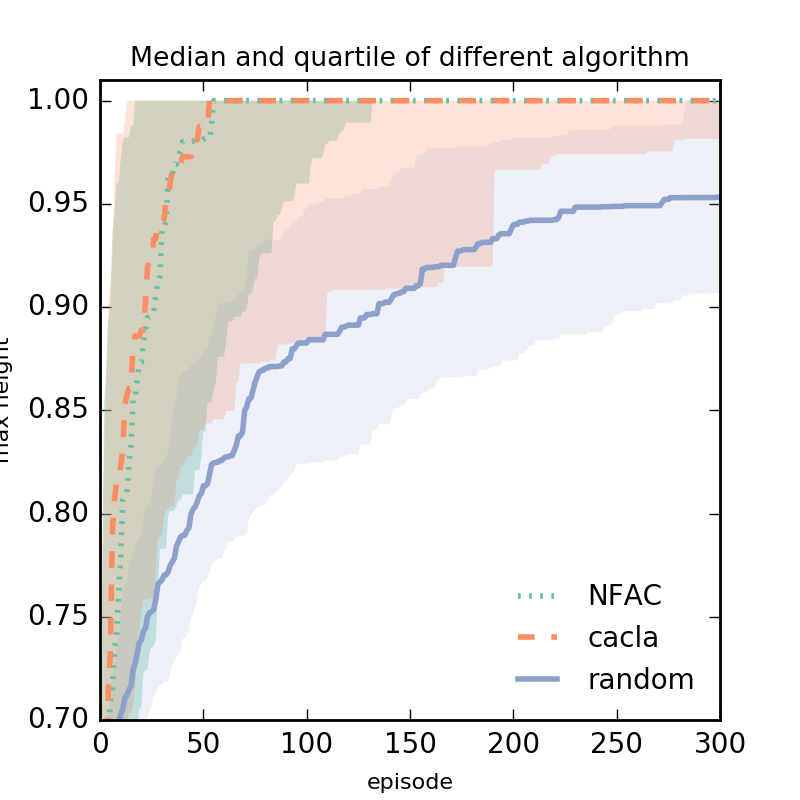
\includegraphics{result_plotting/adacrobot-1ddl.png}
		\caption{..}
		\label{image:adacrobot}
	\end{center}
\end{figure}
Median performance of cacla and NFAC are equivalent. However NFAC is more stable as the lower quartile reach the max performance
at episode 150 where 300 is needed with cacla.

Statistics have been made over 150 different runs after meta-parameters optimization for each algorithms.

\DRAFT{
\begin{itemize}
 \item Acrobot 1DDL
 \begin{itemize}
  \item Cacla
  \item NFAC
 \end{itemize}
 
 \item Cartpole
  \begin{itemize}
  \item Cacla
  \item NFAC
 \end{itemize}
\end{itemize}
}

\cite{Antos2008}


% ****************************************************************************
% BIBLIOGRAPHY AREA
% ****************************************************************************

\begin{footnotesize}

% IF YOU DO NOT USE BIBTEX, USE THE FOLLOWING SAMPLE SCHEME FOR THE REFERENCES
% ----------------------------------------------------------------------------
% \begin{thebibliography}{99}
% 
% % For books
% \bibitem{Haykin_book} S. Haykin, editor. \emph{Unsupervised Adaptive Filtering vol.1 : Blind Source Separation}, John Willey ans Sons, New York, 2000.
% 
% % For articles
% \bibitem{DelfosseLoubaton_article}N. Delfosse and P. Loubaton, Adaptibe blind separation of sources: A deflation
% approach, \emph{Signal Processing}, 45:59-83, Elsevier, 1995.
% 
% % For paper in proceedings published as serie books (LNCS,...)
% \bibitem{CrucCichAmari_bookproceedings} S. Cruces, A. Cichocki and S. Amari, The minimum entropy and cumulants based contrast functions for blind source extraction. In J. Mira and A. Prieto, editors, proceedings of the 6$^{th}$ \emph{international workshop on artificial neural networks} ({IWANN} 2001), Lecture Notes in Computer Science 2085, pages 786-793,
% Springer-Verlag, 2001.
% 
% % For paper in conference proceedings
% \bibitem{VrinsArchambeau_proceedings} F. Vrins, C. Archambeau and M. Verleysen, Towards a local separation performances estimator using common ICA contrast functions? In M. Verleysen, editor, \emph{proceedings of the $12^{th}$
% European Symposium on Artificial Neural Networks} ({ESANN} 2004),
% d-side pub., pages 211-216, April 28-30, Bruges (Belgium), 2004.
% 
% % For Technical Report
% \bibitem{Stone_TechRep} J. V. Stone and J. Porrill, Undercomplete independent component analysis for signal separation and dimension
% reduction. Technical Report, Psychology Department, Sheffield
% University, Sheffield, S10 2UR, England, October 1997.
% \end{thebibliography}
% ----------------------------------------------------------------------------

% IF YOU USE BIBTEX,
% - DELETE THE TEXT BETWEEN THE TWO ABOVE DASHED LINES
% - UNCOMMENT THE NEXT TWO LINES AND REPLACE 'Name_Of_Your_BibFile'

\bibliographystyle{unsrt}
\bibliography{../PhD.bib}

\end{footnotesize}

% ****************************************************************************
% END OF BIBLIOGRAPHY AREA
% ****************************************************************************

\end{document}
